\section{Code Description}

  \subsection{C Modules}

    \subsubsection{\texttt{geom}}

      This is a rewrite of the 3D python geometry library I used last year for
      the second COSC363 assignment.  Just simple 3D geometry stuff to make
      working with points and vectors easier.  Now also includes simple 3x3
      matrix computations as well.

    \subsubsection{\texttt{view}}

      This module mainly takes care of the display and reshape functions and
      setting up what display type is used for the models along with all the
      OpenGL initialisation.

    \subsubsection{\texttt{player}}

      This module simply represents the cameras viewpoint and handles moving
      this around when the movement keys or mouse are used.

    \subsubsection{\texttt{controller}}

      This module takes care of calling all the other initialise functions then
      takes the input and converts it to the correct function calls.

    \subsubsection{\texttt{lights}}

      This module takes care of the light initialisation and display.

    \subsubsection{\texttt{shaders}}

      This module handles the loading and changing of shaders.

    \subsubsection{\texttt{sphere}}

      This module uses subdivision of an icosahedron as provided by halma from
      \href{http://www.3dbuzz.com/vbforum/showthread.php?118279-Quick-solution-for-making-a-sphere-in-OpenGL}
      {http://www.
      3dbuzz.com/vbforum/showthread.php?
      118279-Quick-solution-for-making-a-
      sphere-in-OpenGL}

    \subsubsection{\texttt{texture}}

      This module handles the generation of the pencil shading texture.

    \subsubsection{\texttt{model}}

      This folder contains all the modules related to the half-edge data
      structure and the model loading and displaying.

    \subsubsection{\texttt{time}}

      This module provided both POSIX and Windows implementations of a high
      resolution timer to keep the movement constant.

    \begin{figure}
      \centering
      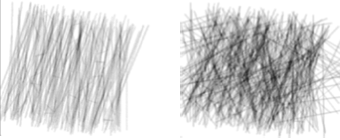
\includegraphics[width=0.45\textwidth]{images/graphite}
      \caption{Pencil strokes generated by Sousa and Buchanan's method.}
      \label{graphite}
    \end{figure}

  \newpage

  \subsection{Shaders}
    
    All the shaders are contained in the \texttt{shaders} folder.  These are all
    simply named with what they do.

  \subsection{Controls}
    
    All keys listed below must be lowercase when pushed.
    
    \subsubsection{Looking}
      
      Hold down the left mouse button and use the mouse to look around.

    \subsubsection{Navigation}

      Use \emph{A}, \emph{W}, \emph{S}, \emph{D}, \emph{Z} and \emph{the
      spacebar} to move the viewpoint left, forwards, back, right, up and down
      respectively.

    \subsubsection{Other}
      \begin{description}
        \setlength{\topsep}{0pt}
        \setlength{\parskip}{0pt}
        \setlength{\partopsep}{0pt}
        \setlength{\parsep}{0pt}
        \setlength{\itemsep}{0pt}

        \item[Q]{ Toggle rotation of the model. }

        \item[E]{ Toggle showing the FPS in the console. }

        \item[R]{ Switch to the next shader model. }

      \end{description}
